\section{Experimental Study}
\label{ch:experiments}

The experiments use seeded synthetic uncertainty so that every local measurement
can be regenerated. The static nonlinear benchmark compares nominal, scenario,
unbiased KDE, and local shifted Epanechnikov constraints. Gaussian, bimodal, skewed, and
heavy-tailed samples are used to separate parametric assumptions from the residual
space approximation. A logarithmic bandwidth sweep and a sample-size sweep assess
stability. Joint constraints compare equal Boole allocation with maximum-violation
and log-sum-exp constructions.

The second application is a canonical two-generator energy-dispatch model with a
documented two-mode renewable forecast-error mixture with mode weights $0.6$ and
$0.4$, means $-0.25$ and $0.35$, and standard deviations $0.10$ and $0.15$. It is a transparent
synthetic proxy, not a claim to reproduce a particular utility dataset. The
uncertain constraint in this adapter is the balance residual; generator-capacity
constraints are deterministic. The same train/test split, objective, violation,
runtime, and gap fields are used as in the static experiment.

The lunar stages in rendered Chapter~6 are run with the local SciPy Euler
collocation proxy on an 11-node mesh. The nominal transcription returned objective
$29.8052$; subsequent robust stages were retained even when SLSQP reported
failure. Published values reported by \citet{keil2020,keil2021} are used
only as external comparisons and are not merged with local measurements. All
numerical claims below are taken from `results/summary.csv` and the corresponding
JSON records. The benchmark seeds are $20260906$ through $20260910$ for the
static, dispatch, joint, sensitivity, and lunar records, respectively.

\begin{center}
  \textbf{Table:} Local static benchmark results for the Gaussian uncertainty case.
  The independent test set contains 4,000 samples and $\varepsilon=0.1$.
  \label{tab:local-static-results}
  \begin{tabular}{lrrr}
    \toprule
    Method & Objective & $\widehat v_{\rm test}$ & Gap \\
    \midrule
    Nominal & 0.0234 & 0.5180 & -0.4180 \\
    Scenario & 0.6134 & 0.0015 & 0.0985 \\
    Unbiased KDE & 0.1981 & 0.0620 & 0.0380 \\
    Local shifted Epanechnikov & 0.3071 & 0.0193 & 0.0808 \\
    \bottomrule
  \end{tabular}
\end{center}

The nominal solution violates the target substantially. Scenario constraints are
safe but expensive. The unbiased KDE and the local shifted Epanechnikov surrogate
are feasible on this Gaussian split. The local surrogate is not Keil's
Split--Bernstein estimator and no theorem is transferred to it. Across the
bimodal, skewed, and heavy-tailed samples, unbiased/local test violations were
$(0.0150,0.0003)$, $(0.1053,0.0700)$, and $(0.0613,0.0405)$, respectively. The
skewed unbiased run exceeds $\varepsilon$, so this experiment supplies no
unconditional safety certificate.

Figure~\ref{fig:static-violations} reports the independent test violations for
all four residual laws. The dashed line is the design target, not a confidence
bound. Figure~\ref{fig:static-tradeoff} places the same solutions in objective--
violation space; points to the left of the line satisfy the empirical target on
this split. These plots are descriptive diagnostics and do not establish a
finite-sample guarantee.

\begin{figure}[tb]
  \centering
  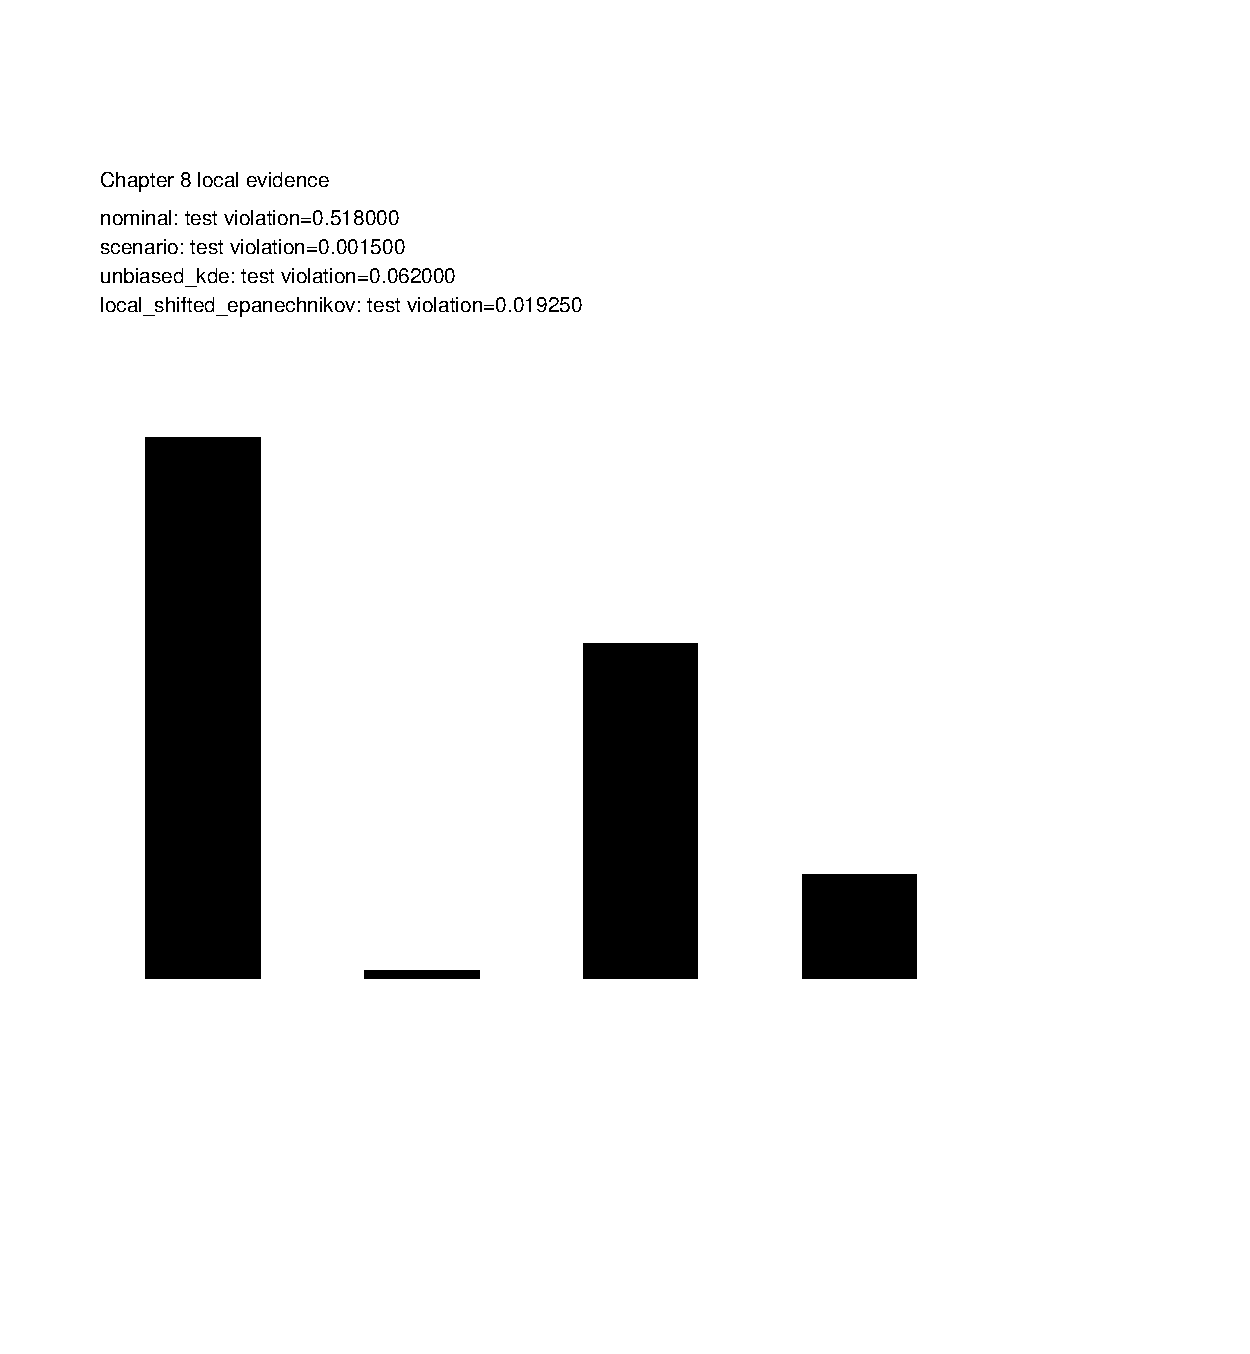
\includegraphics[width=0.94\textwidth]{kap08/figures/fig_static_test_violation}
  \caption{Independent test violation for the static nonlinear benchmark
  ($N_{\mathrm{train}}=250$, $N_{\mathrm{test}}=4000$, $\varepsilon=0.1$).
  Each panel uses one seeded residual law; the dashed line marks the target.}
  \label{fig:static-violations}
\end{figure}

\begin{figure}[tb]
  \centering
  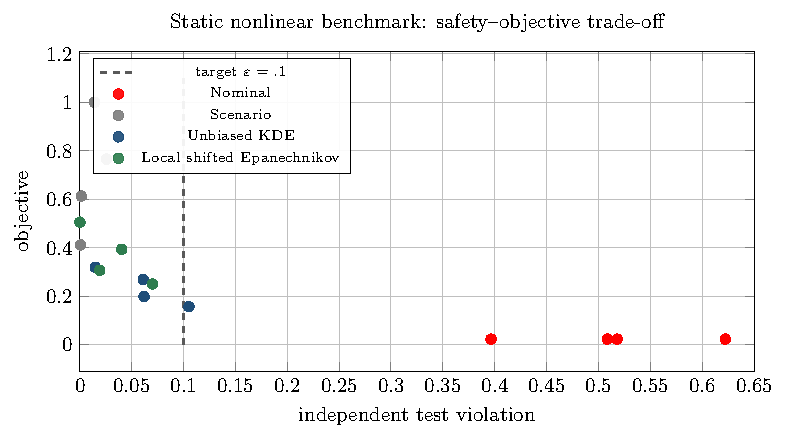
\includegraphics[width=0.88\textwidth]{kap08/figures/fig_static_tradeoff}
  \caption{Objective versus independent test violation for the four static
  residual laws. The vertical dashed line marks $\varepsilon=0.1$.}
  \label{fig:static-tradeoff}
\end{figure}

The residual-estimator diagnostics are shown in Figure~\ref{fig:sensitivity}.
They vary the bandwidth and training size on a separate fixed synthetic scalar
residual split while holding its test samples fixed. The curves therefore measure
estimator sensitivity rather than end-to-end optimizer variability; the numerical
ranges are reported in Chapter~9.

\begin{figure}[tb]
  \centering
  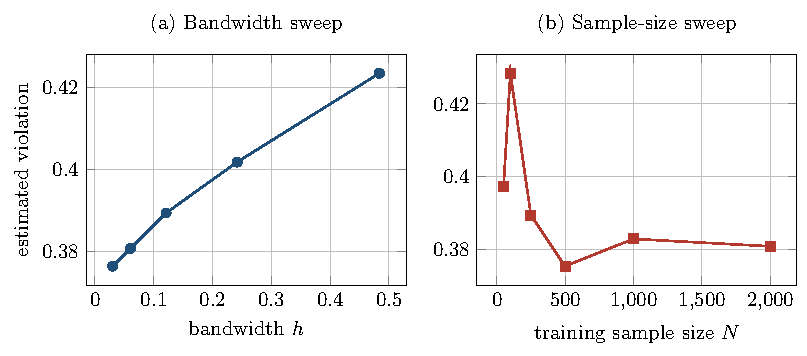
\includegraphics[width=0.90\textwidth]{kap08/figures/fig_sensitivity}
  \caption{Sensitivity of the residual violation estimate to bandwidth and
  training sample size for a fixed synthetic scalar residual split.}
  \label{fig:sensitivity}
\end{figure}

\pagebreak
\begin{samepage}
For the joint experiment, the recorded equal-allocation and exact-maximum
statistics coincide on this sample, giving a joint test violation of $0.5530$;
the $\tau=0.1$ log-sum-exp statistic gives $0.5745$. The equal Boole allocation
is recorded as a comparison and was not enforced as a separate optimized set of
component constraints. Smoothing increased the observed joint violation in this
statistic comparison. The dispatch adapter optimized each method: objectives were $928.57$,
$935.39$, $933.92$, and $934.89$ for nominal, scenario, unbiased KDE, and local
shifted Epanechnikov, with test violations $0.5788$, $0.0060$, $0.0398$, and
$0.0110$.
\end{samepage}

The lunar stage records were, in stage order, $(J,\widehat v_{\rm test})
=(29.8052,0.5143)$ for nominal, $(29.8052,0.5143)$ for worst-case,
$(31.3685,0.0255)$ for scenario, $(32.4400,0.1128)$ for unbiased KDE, and
$(32.4400,0.0548)$ for the local shifted Epanechnikov surrogate. Only the
nominal stage reported solver success in this local transcription; the failed
stages remain in the artifact and are not treated as feasible solutions. The
terminal-position risk level is $\varepsilon_a=0.1$. These results are not a
reproduction of the LGR/IPOPT experiment of Keil et al.; the local Euler mesh,
horizon, and solver are different, so the cost comparison is diagnostic rather
than a performance claim.
